%----------------------------------------------------------------------------------------
%	PACKAGES AND THEMES
%----------------------------------------------------------------------------------------
\documentclass[aspectratio=169,xcolor=dvipsnames]{beamer}
\usetheme{SimplePlus}

\usepackage{algorithm,algorithmic}
\usepackage{hyperref}
\usepackage{graphicx} % Allows including images
\usepackage{booktabs} % Allows the use of \toprule, \midrule and \bottomrule in tables

\renewcommand{\algorithmicrequire}{\textbf{Input:}}
\renewcommand{\algorithmicensure}{\textbf{Output:}}

%----------------------------------------------------------------------------------------
%	TITLE PAGE
%----------------------------------------------------------------------------------------

\title[short title]{A multi-objective adaptive evolutionary algorithm to extract communities in networks} % The short title appears at the bottom of every slide, the full title is only on the title page

\author[Haris-Ali] {Haris Karim Ladhani \& Ali Hamza}

\institute[HU-CI] % Your institution as it will appear on the bottom of every slide, may be shorthand to save space
{
    CS 451 - Computational Intelligence \\
    Habib University % Your institution for the title page
}
\date{\today} % Date, can be changed to a custom date


%----------------------------------------------------------------------------------------
%	PRESENTATION SLIDES
%----------------------------------------------------------------------------------------

\begin{document}

\begin{frame}
    % Print the title page as the first slide
    \titlepage
\end{frame}

\begin{frame}{Overview}
    % Throughout your presentation, if you choose to use \section{} and \subsection{} commands, these will automatically be printed on this slide as an overview of your presentation
    \tableofcontents
\end{frame}

%------------------------------------------------
\section{Introduction}
%------------------------------------------------

\begin{frame}{Introduction}
\begin{itemize}
    \item Many complex systems such as social networks, protein networks can be abstracted into networks i.e. large graphs
    \item Analysis techniques of these networks require studying various patterns within them
    \item Common patterns include recognizing substructures within the graphs such as cliques
    \item This paper analyzes a social network data set and attempts to find communities within it via a genetic algorithm to reduce the complexity of the problem
    \item Communities can be defined by various definitions therefore the paper uses two fitness functions.
    \item \textit{max(internal links) and min(external links)}
\end{itemize}

\end{frame}

\begin{frame}{Problem Description}
    The problem at hand from a CS theoretical point of view is simply a clique, or sub graph, finding problem. 
    %How to find a clique in a graph
    %Clique finding - formal algorithm
    %NP Complete
\end{frame}

\begin{frame}{Motivation}
    %Genetic algorithm part of FYP 
    %Looking for cliques in protient networks
    %Opportunity to explore non-protein network solutions
\end{frame}

%------------------------------------------------

%------------------------------------------------
\section{Genetic Algorithm Formulation}
%------------------------------------------------

\begin{frame}{Encoding Scheme}
    
\end{frame}

%------------------------------------------------
\begin{frame}{Chromosome Representation}
    
\end{frame}

%------------------------------------------------

\begin{frame}{Selection}
   
\end{frame}

%------------------------------------------------

\begin{frame}{Crossover}
   
\end{frame}

%------------------------------------------------

\begin{frame}{Mutation}
   
\end{frame}

%------------------------------------------------

\begin{frame}{Fitness Function}
   
\end{frame}

\begin{frame}{Elitism}
    
\end{frame}
%------------------------------------------------

\begin{frame}{Algorithm}
    \begin{algorithm}[H]
        \begin{algorithmic}[1]
        \STATE \textbf Input: Adaptive parameters: adaptive crossover probability $p_{c}$ of
        population $P$, adaptive mutation probability $p_{m}$ of population $P$
        \STATE $P \leftarrow $ Initialize Population
        \STATE $E \leftarrow $ Initialize Elite Gene Pool
        \STATE While Termination != true;
        \STATE $P_{parent} \leftarrow Select(P)$
        \STATE $p_{c}, p_{m} \leftarrow Adaptive();$
        \STATE $p_{cross} \leftarrow Crossover(P_{parent}, p_{c})$
        \STATE $p_{cross} \leftarrow Mutation(P_{cross}, p_{m})$
        \STATE $P \leftarrow Update(P_{child})$
        \STATE Update Elite Gene Pool
        \STATE End;
        \STATE \textbf{Output} The results of community detection //{Transforming the most adaptable non-inferior solutions from the elite gene pool into community detection results}
        \end{algorithmic}
        \caption{Framework of F-SGCD Algorithm}
        \label{alg:seq}
    \end{algorithm}
\end{frame}

%------------------------------------------------

\begin{frame}{Experiments on synthetic LFR networks}
    \begin{columns}
        % Column 1
        \begin{column}{0.5\textwidth}
                It can be observed that the algorithm performs relatively better than the others
        \end{column}
        % Column 2    
        \begin{column}{0.5\textwidth}
            \begin{figure}
            \centering
                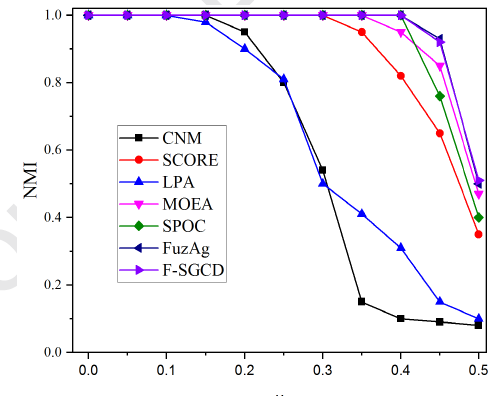
\includegraphics[width=0.8\textwidth]{synthetic-LFR.PNG}
                \caption{Comparison of F-SGCD and other algorithm.}
            \end{figure}
        \end{column}
    \end{columns}
\end{frame}

%------------------------------------------------

\begin{frame}{Experiments on synthetic real-world networks}
    \begin{columns}
        \begin{column}{0.5\textwidth}
            \begin{figure}
            \centering
                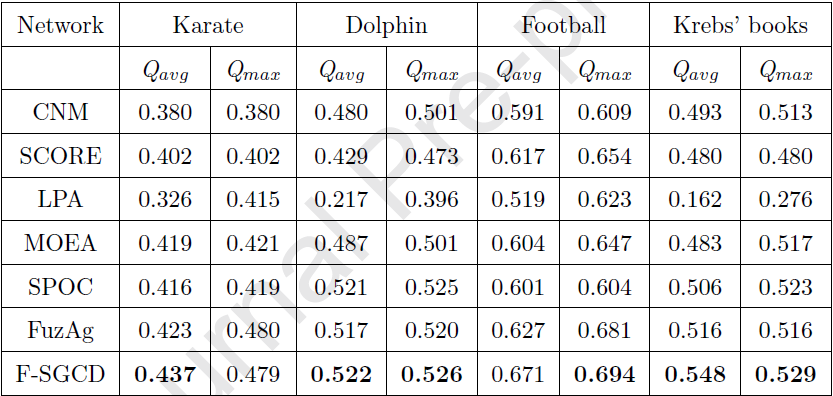
\includegraphics[width=1\textwidth]{synthetic-realworld.PNG}
                \caption{Q values of the eight compared algorithms on four real-world networks, averaging
                over 20 runs.}
            \end{figure}
        \end{column}
    \end{columns}
\end{frame}

%------------------------------------------------

\begin{frame}{Network hierarchy of Pareto solution}
    \begin{itemize}
        \item Hierarchal modularity \\
        In a hierarchical modular network, many small-scale vertices with dense internal connections are loosely connected, and thus forming a larger-scale topology module. This topological structure is arranged in hierarchical order, and the network that generates modules iteratively is called hierarchical network.
        \item Bottlenose Dolphins
    \end{itemize}
\end{frame}

%------------------------------------------------

\begin{frame}{References}
    % Beamer does not support BibTeX so references must be inserted manually as below
    \footnotesize{
        \begin{thebibliography}{99}
            \bibitem[Li-Cao-Ding-Li, 2020]{p1} Qi Li, Zehong Cao, Weiping Ding, Qing Li (2020)
            \newblock A multi-objective adaptive evolutionary algorithm to extract communities in networks
            \newblock \emph{Swarm and Evolutionary Computation} 100629.
        \end{thebibliography}
    }
\end{frame}

%------------------------------------------------
\section{Conclusion}
%------------------------------------------------

\begin{frame}{Conclusion}
    \begin{itemize}
        \item Normalized Mutual Information (NMI) \\
        It is used to measure the similarity between the detected communities and the known communities. Given two partitions $A$ and $B$ of a network in communities, let $C$ be the confusion matrix whose element $C_{ij}$ is the number of nodes of community $i$ of the partition $A$ that are also in the community $j$ of the partition $B$.
        \item Modularity \\
        It is a criterion for evaluating the quality of community detection.
    \end{itemize}
\end{frame}
%------------------------------------------------

% \begin{frame}{References}
%     % Beamer does not support BibTeX so references must be inserted manually as below
%     \footnotesize{
%         \begin{thebibliography}{99}
%             \bibitem[Smith, 2012]{p1} John Smith (2012)
%             \newblock Title of the publication
%             \newblock \emph{Journal Name} 12(3), 45 -- 678.
%         \end{thebibliography}
%     }
% \end{frame}

%------------------------------------------------

% \begin{frame}
%     \Huge{\centerline{\textbf{The End}}}
% \end{frame}

%----------------------------------------------------------------------------------------

\end{document}